%%%%%%%%%%%%%%%%%%%%%%%%%%%%%%%%%%%%%%%%%
% University Assignment Title Page 
% LaTeX Template
% Version 1.0 (27/12/12)
%
% This template has been downloaded from:
% http://www.LaTeXTemplates.com
%
% Original author:
% WikiBooks (http://en.wikibooks.org/wiki/LaTeX/Title_Creation)
%
% License:
% CC BY-NC-SA 3.0 (http://creativecommons.org/licenses/by-nc-sa/3.0/)
%
%%%%%%%%%%%%%%%%%%%%%%%%%%%%%%%%%%%%%%%%%
%\title{Title page with logo}
%----------------------------------------------------------------------------------------
%	PACKAGES AND OTHER DOCUMENT CONFIGURATIONS
%----------------------------------------------------------------------------------------

\documentclass[12pt]{article}
\usepackage[english]{babel}
\usepackage[utf8]{inputenc}
\usepackage{amsmath}
\usepackage{color}
\usepackage[explicit]{titlesec}
\usepackage[hyphens,spaces,obeyspaces]{url}
\usepackage{graphicx}
\usepackage{caption}
\usepackage{subcaption}
\usepackage{grffile}
\usepackage{listings}
\usepackage{placeins}
\usepackage[ 
    urldate=long, 
    sorting=none 
]{biblatex} 
\addbibresource{mybib.bib} 

\usepackage{booktabs}
\usepackage{tabularx}

\begin{document}

\begin{titlepage}

\newcommand{\HRule}{\rule{\linewidth}{0.5mm}} % Defines a new command for the horizontal lines, change thickness here

\center % Center everything on the page
 
%----------------------------------------------------------------------------------------
%	HEADING SECTIONS
%----------------------------------------------------------------------------------------

\textsc{\LARGE University of St Andrews}\\[1.5cm] % Name of your university/college
\textsc{\Large Computer Graphics}\\[0.5cm] % Major heading such as course name
\textsc{\large CS4102}\\[0.5cm] % Minor heading such as course title

%----------------------------------------------------------------------------------------
%	TITLE SECTION
%----------------------------------------------------------------------------------------

\HRule \\[0.4cm]
{ \huge \bfseries Ring-Based Distributed System}\\[0.4cm] % Title of your document
\HRule \\[1.5cm]
 
%----------------------------------------------------------------------------------------
%	AUTHOR SECTION
%----------------------------------------------------------------------------------------


\Large \emph{Author:}\\
 \textsc{150008022}\\[1cm] % Your name
 
%----------------------------------------------------------------------------------------
%	DATE SECTION
%----------------------------------------------------------------------------------------

{\large \today}\\[2cm] % Date, change the \today to a set date if you want to be precise

%----------------------------------------------------------------------------------------
%	LOGO SECTION
%---------------------------------------------------------------------------------------


\includegraphics[width = 4cm]{images/standrewslogo.png}
 
%----------------------------------------------------------------------------------------

\vfill % Fill the rest of the page with whitespace

\end{titlepage}

\section*{Goal}

The aim of this practical is to understand the key principles behind various techniques
frequently used for the rendering of 3D objects, and to get hands-on experience with their implementation and manipulation.

\pagenumbering{arabic}
\setcounter{page}{1} 

\section{Running the Program}

The project uses \texttt{maven} for lifecycle and dependency management.
\texttt{LWJGL} was used for this project, which provides a way to use \texttt{OpenGL} from Java. 
OpenGL \textit{may} be a cause of compatibility issues when running, but an early and forward compatible profile was used to minimise the risk of this.

\bigskip
\noindent\textbf{Usage} 

\noindent\texttt{mvn clean install} will compile the project, run all tests, and produce an exectuable jar.

\noindent\texttt{cd target} to enter the directory where the jar has been compiled.

\noindent \texttt{java -jar FaceModelling-jar-with-dependencies.jar} to run the program. Pass the \texttt{-h} flag to see options.

\section{Implementation}

\subsection{Loading Mesh Data}

A \texttt{FaceLoader} instance initialises by parsing the indices (\texttt{mesh.csv}), and the average face coordinates (\texttt{sh\_000.csv}), vertex weighting (\texttt{sh\_ev.csv}), average face colour (\texttt{tx\_000.csv}), and colour weightings (\texttt{tx\_ev.csv}).
The indices are converted from 1-indexed to 0-indexed when being loaded in.
The \texttt{FaceLoader} instance then loads the deltas for both coordinates and colours for each face, calculating the actual coordinates for each vertex of each face.

The arrays of face data are then passed to the \texttt{MeshLoader} which creates a vertex array object (VAO) for each face, and binds a vertex buffer object (VBO) for the vertices, indices, and colours to them.

The use of indices instead of simply listing all coordinates saves on memory as the one vertex can be used in many triangles, as demonstrated in figure \ref{fig:index_mesh}.

\begin{figure}[!ht]
	\centering
	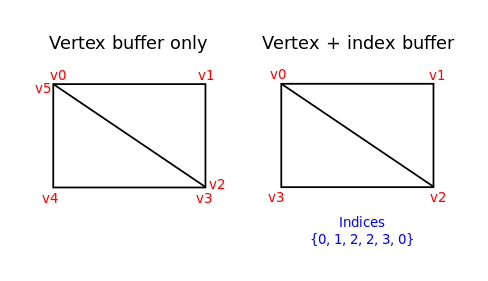
\includegraphics[width=\linewidth]{images/vertex_vs_index}
	\caption{How indices are used when describing meshes.}
	\label{fig:index_mesh}
\end{figure}

\subsection{Depth Testing and Painters Algorithm}

OpenGL does not natively implement painters algorithm for depth testing, and does not expose an API for carrying it out .
Instead, it uses Z-buffers, 
Z-Buffers involve recording the z-index last drawn at each pixel of the window view. 
A pixel with a greater z-index than the current value will be drawn and the z-buffer updated to reflect the new value.
Otherwise the depth test fails and the object will not be drawn at that coordinate.
This functionality is enabled using the \texttt{glEnable(GL11.GL\_DEPTH\_TEST)} call.
An optimisation called early z-testing is often used which is applied earlier on in the rendering pipeline in order to reduce the number of fragments that need to be processed in total.

Painters algorithm and Z-buffers are both viable solutions to the same problem; the former is more computationally expensive while the latter requires more memory.
Z-Buffers are preferred in most cases for modern hardware since memory has become cheaper. 
Painters algorithm also requires additional computation in the case where objects intersect. 
Methods to solve this involve splitting the intersecting shapes and rendering these instead.

A separate renderer was implemented that used painters algorithm.
This renderer was significantly slower both due to the added computation necessary for the painters algorithm, and also due to the fact that the sorting was performed using the CPU rather than the GPU.

The first step involved applying each transformation to the set of coordinates. 
To try improve performance, this task was parallelised using a thread pool.
Then, for each triplet of indices (i.e. each triangle), the maximum Z value was recorded.
Next, maximum z values for each triangle were sorted lowest to highest using a custom \texttt{quicksort} implementation.
The custom implementation was necessary so that every swap performed on the array of maximum z values would also be performed on the indices array, effectively sorting each triangle by maximum z value.
The new indices would then be passed as a VBO for OpenGL, which renders triangles in order of appearance in the indices VBO.

% TODO overlapping tests?

\subsection{Selection Triangle}

The selection triangle is rendered with the three control faces at each vertex.
A left click on the triangle updates the weighting to be used when producing the interpolated face.
This required carrying out ray casting with respect to the mouse position, and was achieved using the steps described by \cite{screenspace}.
Mapping the left click to a position on the selection triangle involved converting from the 2D screen space coordinates to OpenGLs 3D device coordinate system (Figure \ref{fig:screen_coordinates}).

\begin{figure}[!ht]
	\centering
	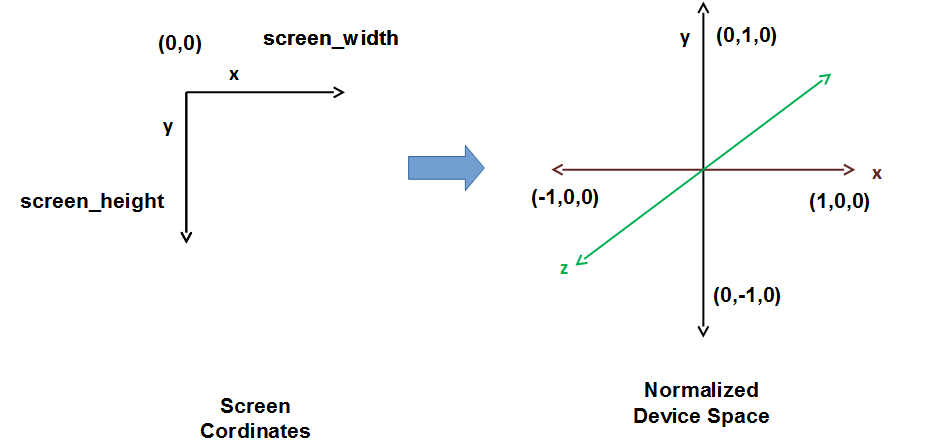
\includegraphics[width=\linewidth]{images/screen_coordinates.png}
    \caption{Converting from screen space to OpenGL \cite{lwjglgamedev}.}
	\label{fig:screen_coordinates}
\end{figure}

We then apply the inverse of the transformation matrices we used to convert to screen space to get the coordinates in world space.
A marker is shown on the triangle to represent the current weighting, and the colour of the marker also reflects the current weighting.
The weightings are calculated using a rearrangement of the following system of equations \cite{barycentric}:

$$
P_x = W_{p1}X_{p1} + W_{p2}X_{p2} + W_{p3}X_{p3} 
$$
$$
P_y = W_{p1}Y_{p1} + W_{p2}Y_{p2} + W_{p3}Y_{p3}
$$
$$
1 = W_{p1} + W_{p2} + W_{p3}
$$

If our user clicks outside the bounds of the selection triangle, a negative weighting would be produced, which we can check for before updating the output face.

\subsection{Interpolated Face}

For each vertex of the face, the coordinates can be calculated using the equations for Barycentric coordinates described above.

\newpage
\section{Summary of Implementation}
\noindent\textbf{Requirements}
\begin{itemize}
    \itemsep0em
    \item  Render faces using index, coordinate, and colour buffers
    \item  Painters algorithm 
    \item  Click triangle to select weighting between different faces
    \item  Interpolate to create face from control faces with weighting
    \item  Flat shading
    \item  Gouraud shading
    \item  Orthographic projection
    \item  Perspective projection
    \item  Adjustable focal length
    \item  Comparison of shading and projection
    \item  Light attention model from lectures
    \item  Adjustable free parameters
    \item  Phongs secularity term in reflectance model
\end{itemize}

\noindent\textbf{Extensions}
\begin{itemize}
\itemsep0em
\item Camera is able to move around 3D world
\item Comparison between painters algorithm and z-buffers 
\item Control faces are also visible during selection
\item Use of OpenGL for optimised rendering
\item Scene graph to render children objects relative to parents
\end{itemize}

\printbibliography

\end{document}
